\let\negmedspace\undefined
\let\negthickspace\undefined
\documentclass[journal]{IEEEtran}
\usepackage[a5paper, margin=10mm, onecolumn]{geometry}
%\usepackage{lmodern} % Ensure lmodern is loaded for pdflatex
% \usepackage{tfrupee} % Include tfrupee package

\setlength{\headheight}{1cm} % Set the height of the header box
\setlength{\headsep}{0mm}     % Set the distance between the header box and the top of the text

\usepackage{gvv-book}
\usepackage{gvv}
\usepackage{cite}
\usepackage{amsmath,amssymb,amsfonts,amsthm}
\usepackage{algorithm}
\usepackage{algorithmic}
\usepackage{graphicx}
\usepackage{textcomp}
\usepackage{xcolor}
\usepackage{txfonts}
\usepackage{listings}
\usepackage{enumitem}
\usepackage{mathtools}
\usepackage{gensymb}
\usepackage{comment}
\usepackage[breaklinks=true]{hyperref}
\usepackage{tkz-euclide} 
\usepackage{listings}
% \usepackage{gvv}                                        
\def\inputGnumericTable{}                                 
\usepackage[latin1]{inputenc}                                
\usepackage{color}                                            
\usepackage{array}                                            
\usepackage{longtable}                
\usepackage{calc}                                             
\usepackage{multirow}                                         
\usepackage{hhline}                                           
\usepackage{ifthen}                             
\usepackage{caption}              
\usepackage{lscape}
\usepackage{subcaption}
\captionsetup{compatibility=false}
% \captionsetup{compactibility=false}
% \usepackage{algpseudocode}
\begin{document}

\bibliographystyle{IEEEtran}
\vspace{3cm}

\title{Experiment 2} 
\author{S A Aravind Eswar and Eshan Sharma}
{\let\newpage\relax\maketitle}

\section{Aim}

Find the RC circuit responce with all the 3 cases below for a square wave input(+5/-5V)
\begin{align*}
    RC=T\\
    RC>>T\\
    RC<<T
\end{align*}

where,

    
$R$ = Resistance

$C$ = Capacitance

$T$ = Time period of the input


\section{Apparatus/Materials needed}
\begin{enumerate}
    \item Bread Board
    \item Resistance (1k$\ohm$ used here)
    \item Capacitance (0.1$\mu F$ used here)
    \item Function Generator
    \item CRO
\end{enumerate}

\section{Theory}

Let the output be $V_l$ at the start of the cycle and $V_u$ in the middle of the cycle after achieving steady-state.

And let $V_i = 5V$
Then,

\begin{align}
    V_l = V_i\brak{1-e^{\frac{-T}{2RC}}} + V_u\,e^{\frac{-T}{2RC}}\\
    V_u = -V_i\brak{1-e^{\frac{-T}{2RC}}} + V_l\,e^{\frac{-T}{2RC}}
\end{align}

Solving the above 2 equations, we get,

\begin{align}
    V_l = -V_i\,\frac{1-e^{\frac{-T}{2RC}}}{1+e^{\frac{-T}{2RC}}}\\
    V_u = V_i\,\frac{1-e^{\frac{-T}{2RC}}}{1+e^{\frac{-T}{2RC}}}
\end{align}

We can observe that,

\begin{enumerate}
    \item If $T>>RC$ then, $V_l\to-V_i$, $V_u\to V_i$
    \item If $T<<RC$ then, $V_l\to 0$, $V_u\to0$
\end{enumerate}

Intuvitively, we can tell, the capacitor will reach the input voltage more time we give it to charge. With less time, capacitor doesn't have much time to charge up and it doesn't give output.

Thus this circuit behaves as a low-pass filter, where lower the frequency, less the attenutaiton.


\section{Procedure}

\begin{enumerate}
    \item Setup a resistor and a capacitor in series with help of a bread board.
    \item Setup the function generator with a square wave of high point as 5V and low point as -5V and with required frequency
    \item Connect the Input(red) to the resistor end and ground to the capacitor.
    \item Connect the first channel of CRO to across the capacitor to oberve it's responce.
    \item Connect the second channel of CRO across the entire circuit to observe the input.
\end{enumerate}

\begin{figure}[!ht]
    \centering
    \resizebox{0.4\textwidth}{!}{%
    \begin{circuitikz}
    \tikzstyle{every node}=[font=\LARGE]
    \draw (7,14.25) to[R,l={ \LARGE 1k$\Omega$}] (10,14.25);
    \draw (10,14.25) to[C,l={ \LARGE 0.1$\mu$F}] (10,11.75);
    \draw (10,14.25) to[short, -o] (12,14.25) ;
    \draw (10,11.75) to[short, -o] (12,11.75) ;
    \draw (10,11.75) to[short, -o] (6.25,11.75) ;
    \draw (7,14.25) to[short, -o] (6.25,14.25) ;
    \node [font=\LARGE] at (6.25,13) {$V_i$};
    \node [font=\LARGE] at (13.5,12.75) {$V_{out}$};
    \end{circuitikz}
    }%
    \caption{Circuit Diagram}
    % \label{fig:my_label}
\end{figure}

\section{Observations}

\subsection{RC = T}

\begin{figure}[!h]
    \centering
    \begin{subfigure}[t]{0.4\textwidth}
        \centering
        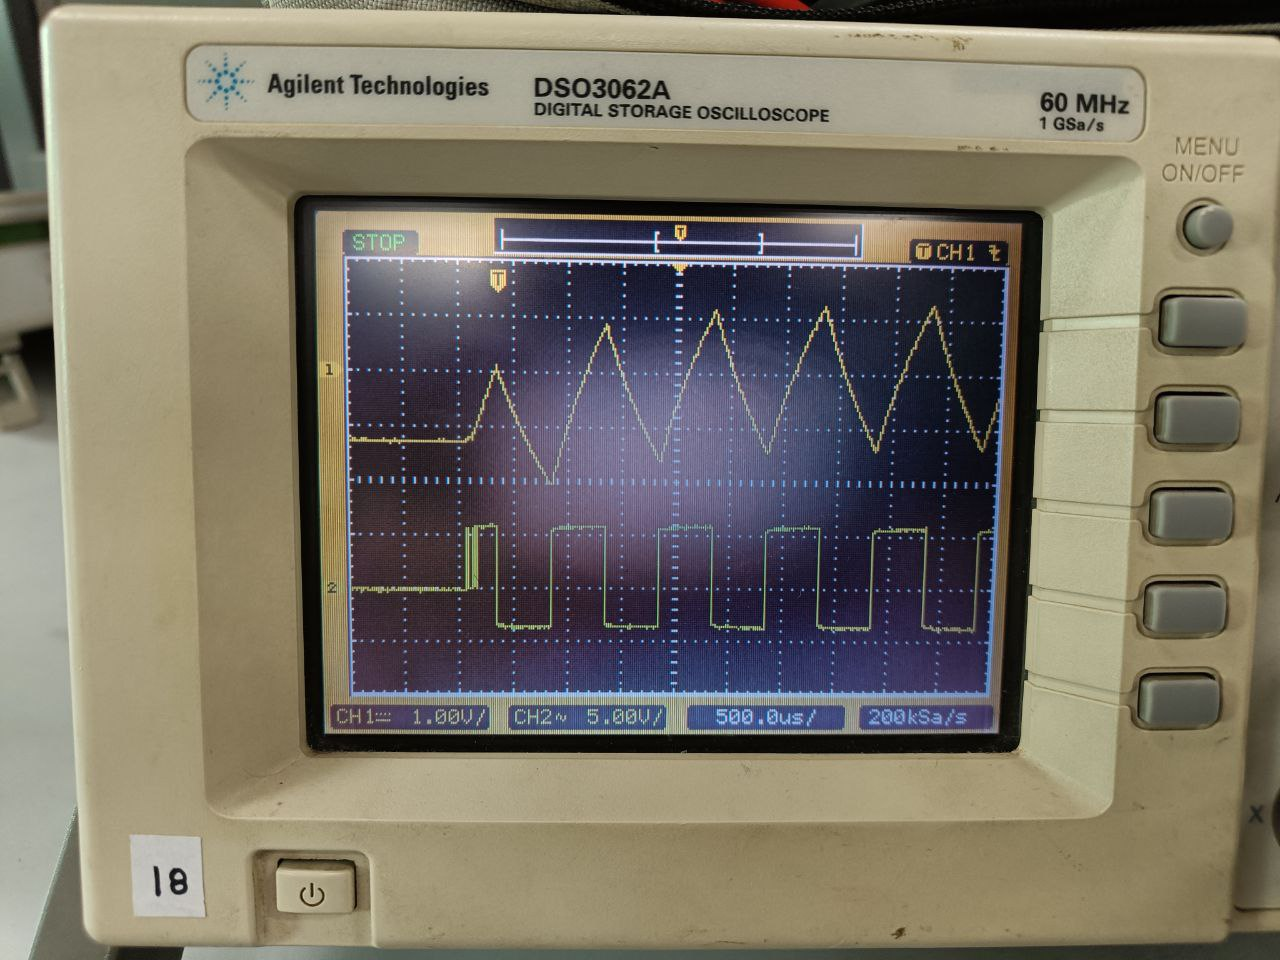
\includegraphics[width=1\columnwidth]{pics/6109622319392604816.jpg}
    \end{subfigure}
    \begin{subfigure}[t]{0.4\textwidth}
        \centering
        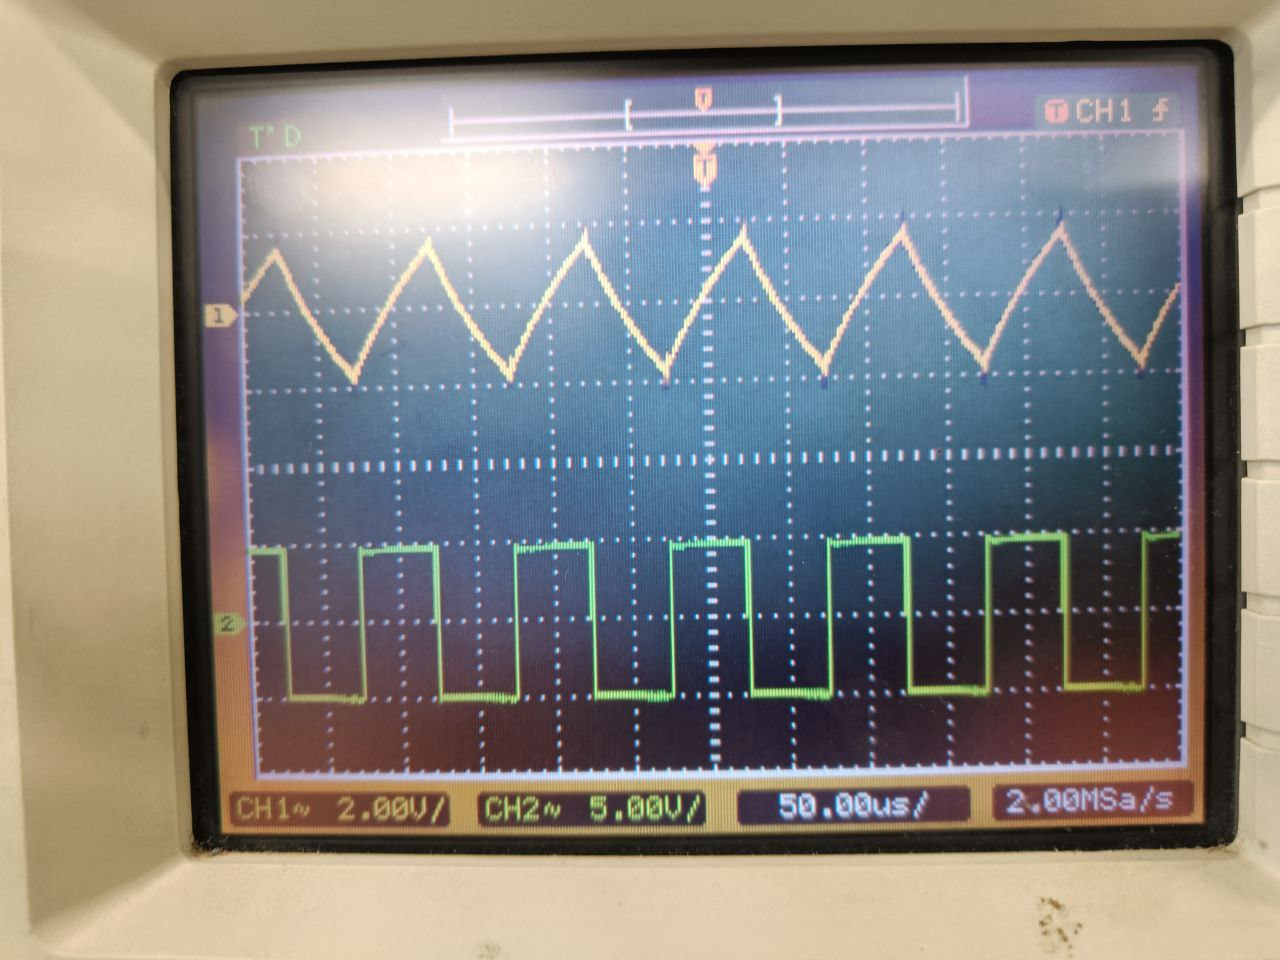
\includegraphics[width=1\columnwidth]{pics/6109622319392604812.jpg}
    \end{subfigure}
    \caption{Transient State and Steady State Observed with CRO}
    %\centering
\end{figure}

\begin{figure}[H]
    \centering
    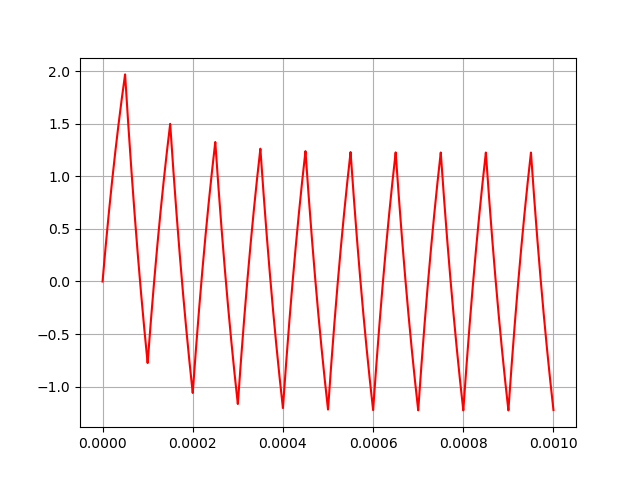
\includegraphics[width=0.6\columnwidth]{figs/fig1.png}
    \caption{Simulation}
\end{figure}

\subsection{$RC >> T$}

\begin{figure}[H]
    \centering
    \begin{subfigure}[t]{0.4\textwidth}
        \centering
        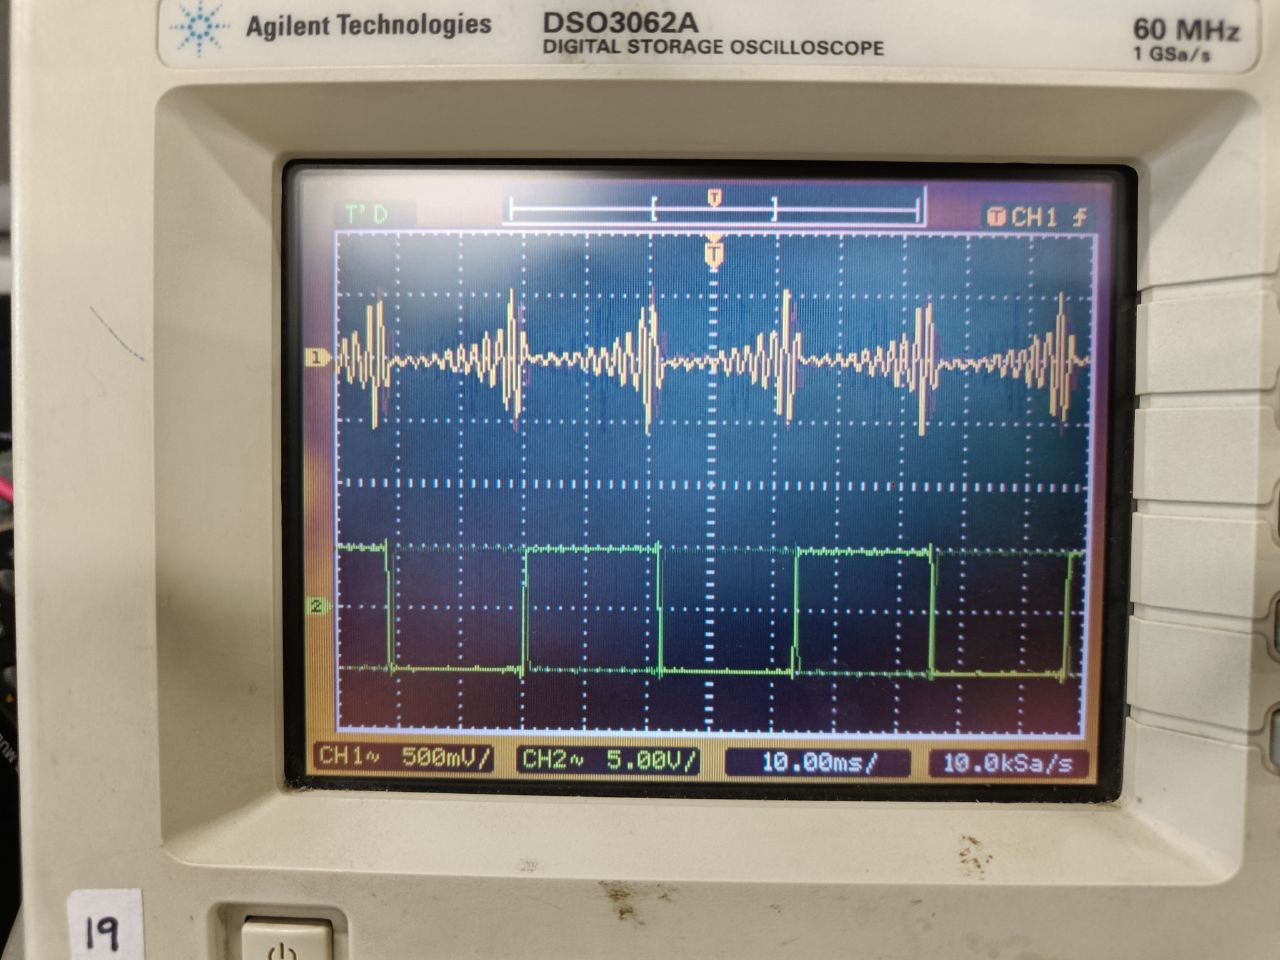
\includegraphics[width=1\columnwidth]{pics/6109622319392604813.jpg}
    \end{subfigure}
    \caption{Steady State Observed with CRO}
    %\centering
\end{figure}

\begin{figure}[H]
    \centering
    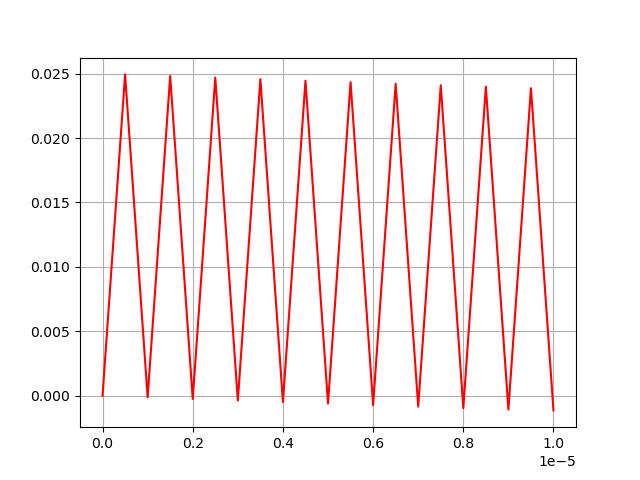
\includegraphics[width=0.6\columnwidth]{figs/fig3.png}
    \caption{Simulation}
\end{figure}

\subsection{$RC << T$}

\begin{figure}[H]
    \centering
    \begin{subfigure}[t]{0.4\textwidth}
        \centering
        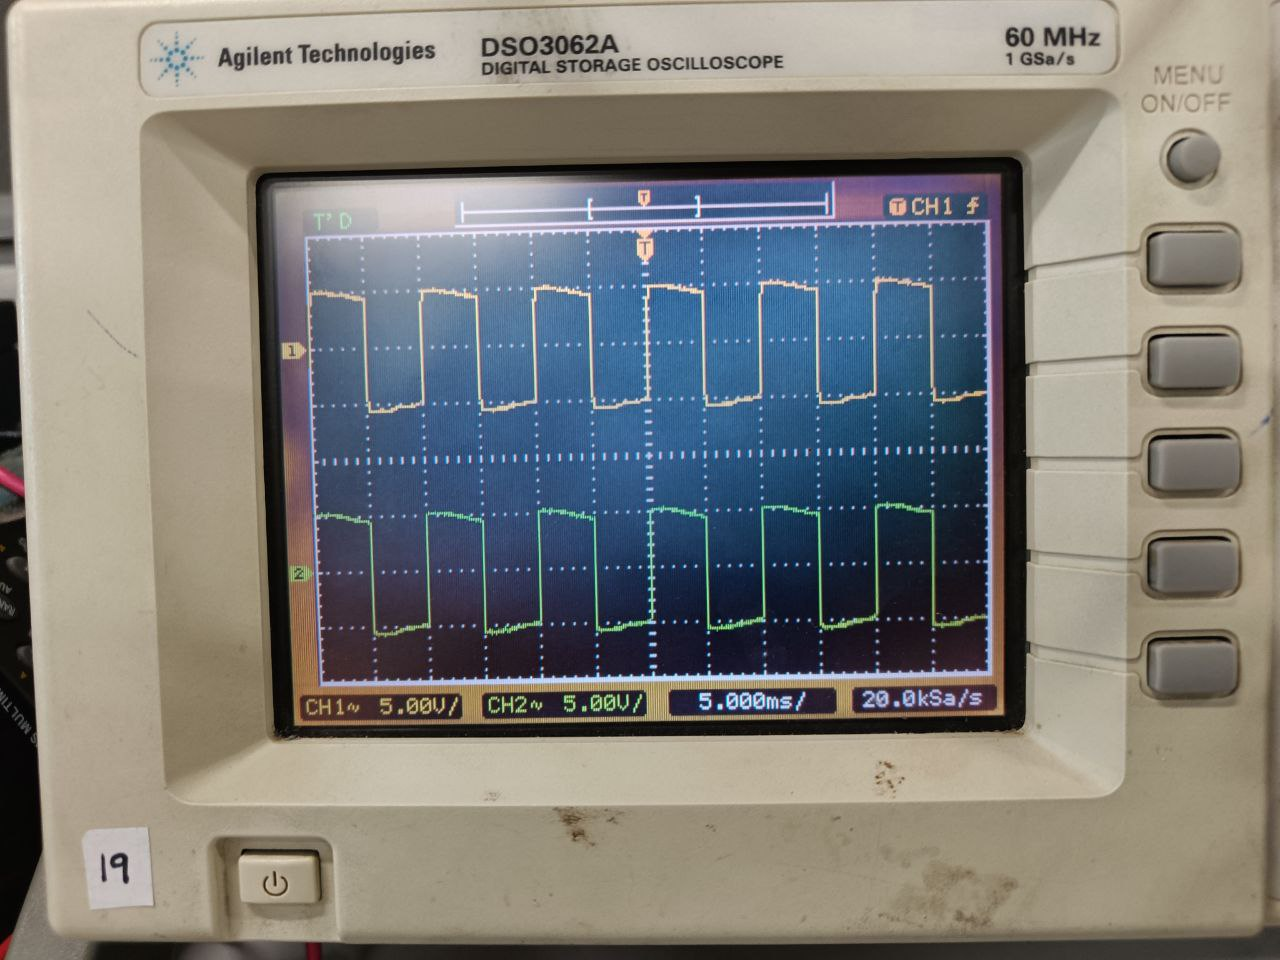
\includegraphics[width=1\columnwidth]{pics/6109622319392604814.jpg}
    \end{subfigure}
    \caption{Steady State Observed with CRO}
    %\centering
\end{figure}

\begin{figure}[H]
    \centering
    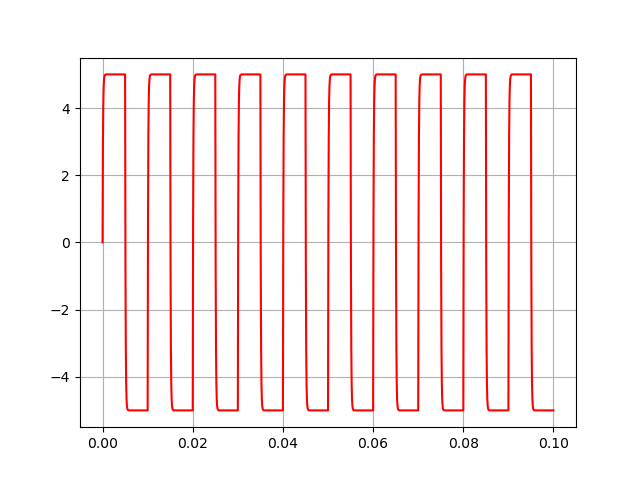
\includegraphics[width=0.6\columnwidth]{figs/fig2.png}
    \caption{Simulation}
\end{figure}

Steady State in case 2 wasn't observed properly due to machine faults.
 
\section{Precautions}

\begin{enumerate}
    \item Use a non polarized capacitor.
    \item Make sure the connections are proper
    \item Don't use very low frequency inputs or the function will not be generated properly by the function generator.
\end{enumerate}

\end{document}
